\documentclass[11pt]{style/nsf}

\usepackage{epsfig}

\usepackage{fontspec}
\setmainfont{Times New Roman}
%\setmainfont{cmunrm} % Computer Modern Roman 
% If using {fontspec} to get actual fonts (like Times New Roman), must compile with LuaLaTeX -or- XeLaTeX.  Not compatible with pdflatex.
% https://tex.stackexchange.com/questions/74496/how-to-use-times-roman-nimbus-roman-with-fontspec-under-linux-and-lualatex/74499
% Setting font size to 11.06 achieves actual font size of 11.019, which will pass Research.Gov.
\usepackage{setspace}
\usepackage{pdfpages} % to include existing pdf files
%\usepackage{hyperref} % Hyperlinks not allowed in NSF documents
\usepackage{enumitem}
\usepackage{graphicx,wrapfig,float} % float to force figure [H]
\graphicspath{{figures/}}
\usepackage[font=small,skip=1pt]{caption} % To remove spacing between figure & its caption
\usepackage{natbib} % for bibliography
\setcounter{secnumdepth}{4} % To allow subsubsubsection (which is called as \paragraph{})
\usepackage{lipsum} % just to generate dummy text


% NSF proposal generation template style file.
% based on latex stylefiles  written by Stefan Llewellyn Smith and
% Sarah Gille, with contributions from other collaborators.

% Updated by Amr Abed, 
% https://github.com/amrabed/NSF-LaTeX-Template

% and updated again by Kristin Poinar 

% Font size needs to be 11 exactly (or larger)
% the 11pt argument actually sets it to 10.95!
% https://tex.stackexchange.com/questions/473838/how-to-set-the-font-size-to-11-5pt

\begin{document}

\fontsize{11.06pt}{14pt}\selectfont 
% Setting font size to 11.06 achieves actual font size of 11.019, which will pass Research.Gov.



% A. Cover Sheet
% The Cover Sheet is now electronically pre-filled by FastLane / Research.gov

% B. Project Summary
% Cannot exceed one page
\newsection{B}
\section*{\hfil Project Summary\hfil}
\vspace{-16pt}
\noindent\hrulefill



%Each proposal must contain a summary of the proposed project not more than {\bf one page in length}. The Project Summary consists of an overview, a statement on the intellectual merit of the proposed activity, and a statement on the broader impacts of the proposed activity.
%The overview includes a description of the activity that would result if the proposal were funded and a statement of objectives and methods to be employed.  
%The Project Summary should be written in the third person, informative to other persons working in the same or related fields, and, insofar as possible, understandable to a scientifically or technically literate lay reader. It should not be an abstract of the proposal.
%If the Project Summary contains special characters it may be uploaded as a Supplementary Document.
%{\bf Project Summaries submitted as a PDF must be formatted with separate headings for the overview, statement on the intellectual merit of the proposed activity, and statement on the broader impacts of the proposed activity}. Failure to include these headings may result in the proposal being returned without review. Additional instructions for preparation of the Project Summary are available in FastLane.\\


\vspace{-8pt}
\subsection*{Overview:} 
\vspace{-7pt}

The key contributions of this template, above what existed already at Amr Abed's repo, are (1) that it is font-size-compatible at Research.gov (size 11.019pt Times New Roman), and (2) that the section headings are configured so that the Project Description (the meaty 15 page part of the full proposal) has its own section heading hierarchy, starting with Section 1 (Motivation) and going forward from there.  Previous versions had Summary as Section 1, Project Description as Section 2, etc. -- which I found annoying, since every heading in the Project Description was preceded by a 2.  These are now fixed, and other small improvements -- like appending ``RO'' (for Research Objective) to certain section headings, and reducing the spacing between paragraphs and section headings to save space -- are added.  Otherwise, much is unchanged from the Amr Abed version.

The proposed work does not involve Arctic fieldwork.




\vspace{-8pt}
\subsection*{Intellectual Merit:}
\vspace{-7pt}

The statement on intellectual merit should describe the potential of the proposed activity to advance knowledge.




\vspace{-8pt}
\subsection*{Broader Impacts:} 
\vspace{-7pt}

The statement on broader impacts should describe the potential of the proposed activity to benefit society and contribute to the achievement of specific, desired societal outcomes.

% C. Table of Contents 
% A Table of Contents is automatically generated for the proposal by FastLane / Research.gov

% D. Project Description
\newpage\newsection{D}
%\title{You may or may not want to display your title; it is not required and takes up space}
\section*{\hfil Project Description \hfil}
\vspace{-16pt}
\noindent\hrulefill
% From solicitation NSF 22-586: 
% https://nsf-gov-resources.nsf.gov/solicitations/pubs/2022/nsf22586/nsf22586.pdf?VersionId=zhHYrr4DGF8u3J8kV3r217ygkg4.fKRM 
%The Project Description section should contain a well-argued and specific proposal for activities that will, over a 5-year period, build a rm foundation for a lifetime of contributions to research and education in the context of the Principal Investigator's organization. The proposed project should aim to advance the employee's career goals and job responsibilities as well as the mission of the department or organization. The Project Description may not exceed 15 pages.
%The Project Description should include: 
% a description of the proposed research project, including preliminary supporting data where appropriate, specific objectives, methods and procedures to be used, and expected significance of the results; 
% a description of the proposed educational activities and their intended impact; 
% a description of how the research and educational activities are integrated or synergistic; 
% a description of other broader impacts, besides the education activities, that will accrue from the project; 
% and results of prior NSF support, if applicable.
%Successful applicants will propose creative, effective research and education plans, along with strategies for assessing these components. The proposed activities should help applicants develop in their careers as both outstanding researchers and educators. While excellence in both education and research is expected, activity of an intensity that leads to an unreasonable workload is not. The research and educational activities do not need to be addressed separately if the relationship between the two is such that the presentation of the integrated project is better served by interspersing the two throughout the Project Description.
%
%
%
%%
% Objectives, Goals, and Tasks
%%
%
% Goals and Objectives are not interchangeable. Think about your research goal, then state your research objectives and the tasks that need to be done to achieve the objectives.
%		Goal – A statement of what you are trying to achieve.
%		Objective(s) – Clearly defined step(s) towards your goal.
%		Tasks – Activities to achieve objective(s)


\vspace{-10pt}
\section{Motivation \& Objectives}

\lipsum[3]

%%%%%%%%%%%%%%%
% RESEARCH OBJECTIVES 
%%%%%%%%%%%%%%%
\begin{enumerate}[label=\textbf{RO~\arabic*.},leftmargin=2cm]

\vspace{-8pt}
\item Achieve bigness

\vspace{-10pt}
\item Achieve fireball power

\vspace{-10pt}
\item Save the prisoner

\end{enumerate}

\lipsum[1]

\setlength{\intextsep}{5pt}  % reduce top/bottom margin from this wrapfig
\begin{wrapfigure}{R}{0.5\textwidth}
	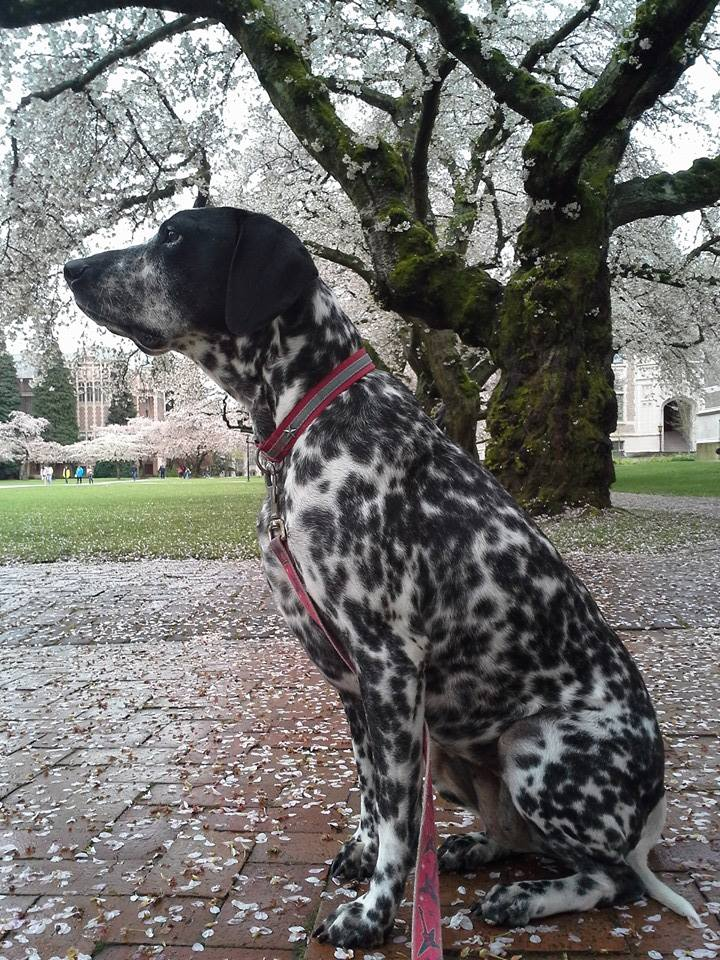
\includegraphics[width=0.5\textwidth]{maggieinthethespring.jpg}
	\caption{\textit{A dog under a blossoming cherry tree.}}
\end{wrapfigure}






\section{Background and motivation}

\lipsum




\section{Proposed Study \& Research Plan}

\lipsum[1]



% Set the subsection to be preceded by RO
\renewcommand{\thesubsection}{\arabic{section}.RO-\arabic{subsection}}

\subsection{Achieve bigness}
\label{sec:RO1}
\vspace{-6pt}

\textit{We will find a mushroom and eat it to grow big.}



\vspace{-10pt}
\subsubsection{Rationale and significance of RO-1}
\vspace{-6pt}

\lipsum[2]




\vspace{-10pt}
\subsubsection{Implementation plan for RO-1}
\vspace{-6pt}


\paragraph*{Task RO-1.A: Run to the right}
\lipsum[1]

\paragraph*{Task RO-1.B: Jump up and hit block}
\lipsum[1]

\paragraph*{Task RO-1.C: Co-occupy the space of the mushroom}
\lipsum[1]

\vspace{-10pt}
\subsubsection{Evaluation plan for RO-1}

\vspace{-8pt}
\paragraph*{Formative evaluation:} 
\lipsum[1]

\vspace{-14pt}
\paragraph*{Summative evaluation:} 
\lipsum[1]


\vspace{-10pt}
\subsubsection{Summary of expected results of RO-1}
\vspace{-6pt}

\lipsum[1]












%Research Objective 2
%•	Task 1 (or R1)
%•	Task 2 (or R2)
%•	…

\bigskip
\vspace{-10pt}
\subsection{Achieve fireball power}
\label{sec:RO2}
\vspace{-6pt}

\textit{We will find a glowing flower and meld with it to get fireball power.}




\vspace{-10pt}
\subsubsection{Rationale and significance of RO-2}
\vspace{-6pt}

\lipsum[2]

\vspace{-10pt}
\subsubsection{Implementation plan for RO-2} 
\label{sec:RO2plan}

\vspace{-6pt}
\paragraph*{Task RO-2.A: Jump onto a turtle}
\lipsum[1]

\vspace{-6pt}
\paragraph*{Task RO-2.B: Kick the turtle into a block}
\lipsum[1]

\vspace{-6pt}
\paragraph*{Task RO-2.C: Occupy the same space as the flower}
\lipsum[1]

\vspace{-10pt}
\subsubsection{Evaluation plan for RO-2}

\vspace{-8pt}
\paragraph*{Formative evaluation:}  
\lipsum[1]


\vspace{-14pt}
\paragraph*{Summative evaluation:}  
\lipsum[1]



\vspace{-10pt}
\subsubsection{Summary of expected results of RO-2}
\vspace{-6pt}

\lipsum[1]





%Research Objective 3
%•	Task 1 (or R1)
%•	Task 2 (or R2)
%•	…

\bigskip
\vspace{-10pt}
\subsection{Save the prisoner}
\label{sec:RO3}
\vspace{-6pt}

\textit{We will find the captured innocent person and save them.}


\vspace{-10pt}
\subsubsection{Rationale and significance of RO-3}
\vspace{-6pt}
\lipsum[2]

\vspace{-10pt}
\subsubsection{Implementation plan for RO-3} 

\vspace{-6pt}
\paragraph*{Task RO-3.A: Enter the castle}
\lipsum[1]

\vspace{-6pt}
\paragraph*{Task RO-3.B: Navigate to the Boss}
\lipsum[1]

\vspace{-6pt}
\paragraph*{Task RO-3.C: Defeat the Boss}
\lipsum[1]

\vspace{-10pt}
\subsubsection{Evaluation plan for RO-3}

\vspace{-8pt}
\paragraph*{Formative evaluation:}  
\lipsum[1]

\vspace{-14pt}
\paragraph*{Summative evaluation:} 
\lipsum[1]


\vspace{-10pt}
\subsubsection{Summary of expected results from RO-3}
\vspace{-6pt}

\lipsum[1]


% Reset subsection numbering back to normal
\renewcommand{\thesubsection}{\arabic{section}.\arabic{subsection}}


\newpage
\section{Broader Impacts of the Proposed Work}
\label{sec:BI}

\lipsum


\section{Timeline}


\begin{figure}[H]
	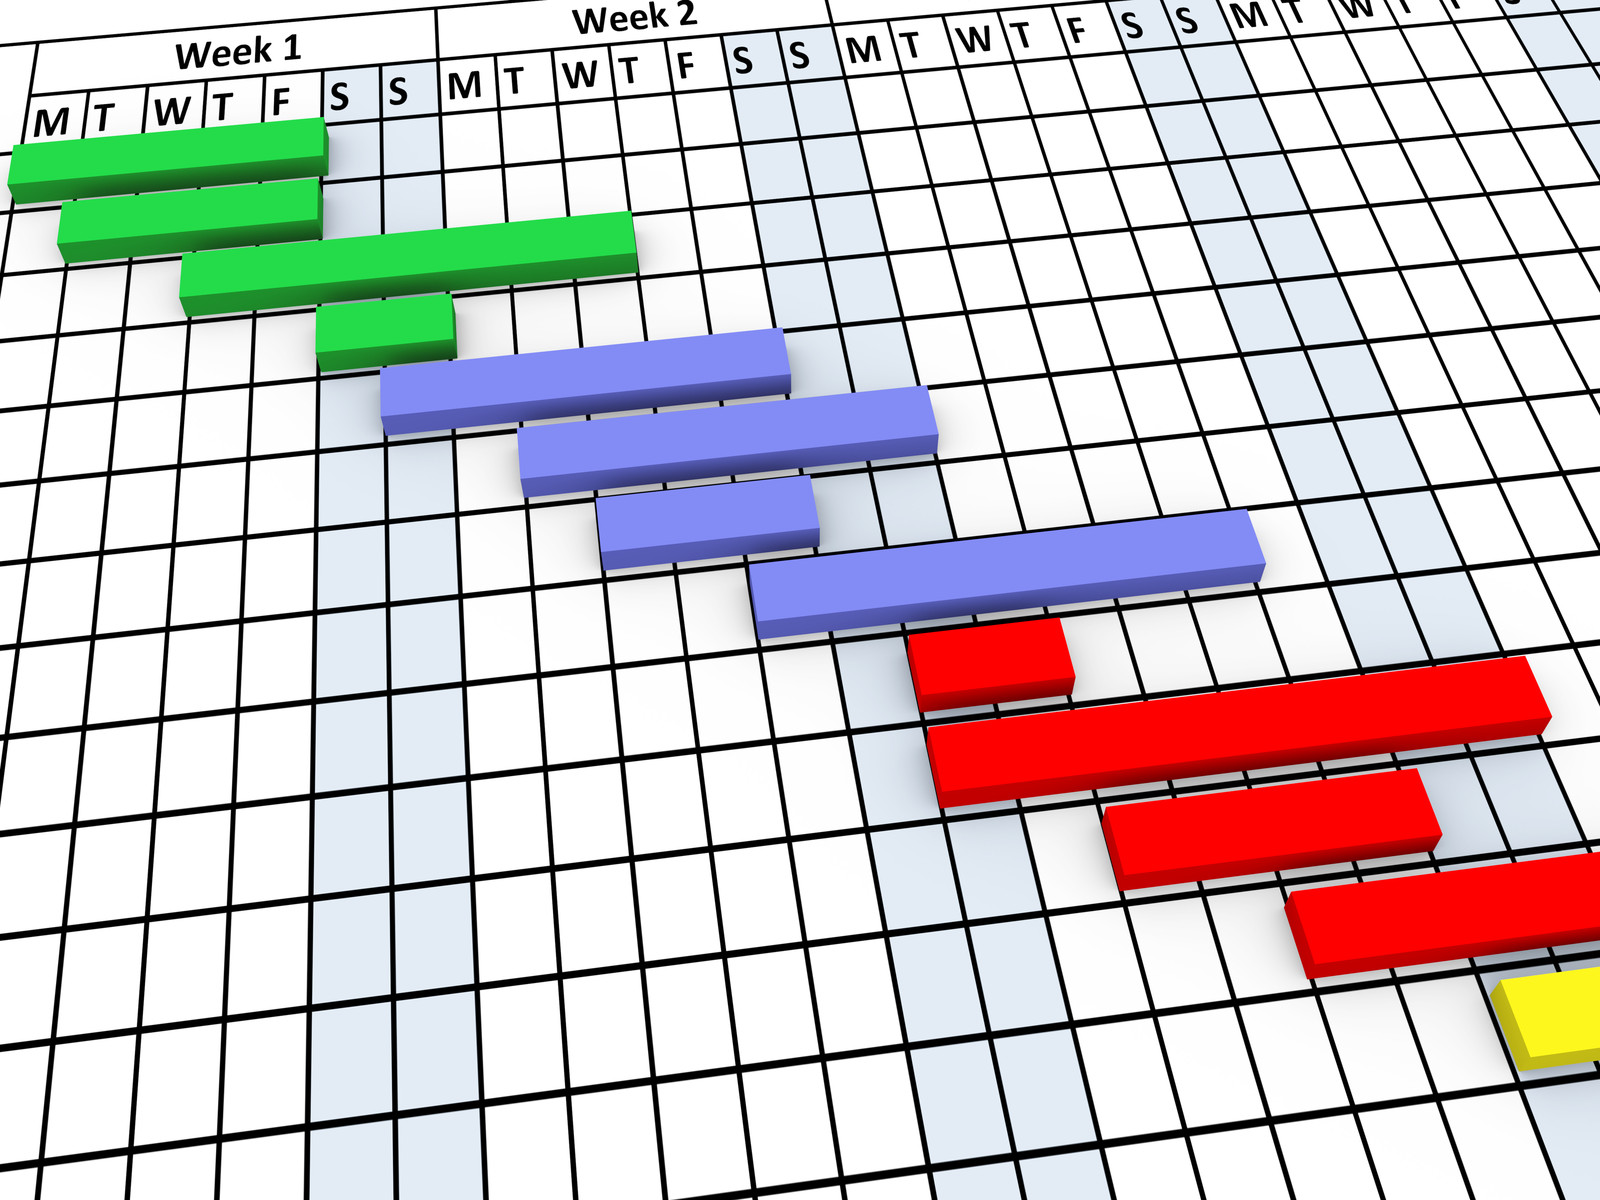
\includegraphics[width=\textwidth]{gantt.jpg}
	\label{fig:gantt}
	\vspace{-10pt}
	\caption{\textit{Timeline for planned completion of the proposed work.}}
\end{figure}

\lipsum[2]


\section{Results from Prior NSF Support}
%If any PI or co-PI identified on the project has received NSF funding (including any current funding) in the past five years, in formation on the award(s) is required, irrespective of whether the support was directly related to the proposal or not.
%In cases where the PI or co-PI has received more than one award (excluding amendments), they need only report on the one award most closely related to the proposal. Funding includes not just salary support, but any funding awarded by NSF. The following information must be provided:\\

\noindent \emph{\underline{Name of PI}}: NSF-Program (Award Number) ``Title of the Project'' (\$AMOUNT, PERIOD OF SUPPORT). 
{\bf Publications:} List of publications resulting from the NSF award. A complete bibliographic citation for each publication must be provided either in this section or in the References Cited section of the proposal); if none, state: ``No publications were produced under this award.'' {\bf Research Products:} evidence of research products and their availability, including, but not limited to: data, publications, samples, physical collections, software, and models, as described in any Data Management Plan.

% evidence of research products and their availability, including, but not limited to: data, publications, samples, physical collections, software, and models, as described in any Data Management Plan.



% E. References Cited
\newpage\newsection{E}
\renewcommand\refname{References Cited}
\bibliography{proposal}

% F. Biographical Sketch(es)
\newpage\newsection{F}
\include{sections/biosketch}

% G. Budget Justification
\newpage\newsection{G}
\section*{\hfil Budget Justification \hfil}
\vspace{-16pt}
\noindent\hrulefill
% No more than 3 pages!!! 

\subsection*{A. Senior Personnel}

\noindent{\bf A1.} The PI

Anticipated salary increases of 3\% are applied in each year following Year 1.


\subsection*{B. Other Personnel}

\noindent{\bf B1. Postdoctoral Associate:} 
\vspace{10pt}

\noindent{\bf B3. Graduate Students:} 
\vspace{10pt}

\noindent{\bf B4. Undergraduate Students: } 

Anticipated salary increases of 3\% are applied in each year following Year 1.




\subsection*{C. Fringe Benefits}
Fringe benefits are calculated at a rate of X\% for faculty, Y\% for graduate students.  

\subsection*{D. Equipment}
Equipment of X, Y, and Z will be purchased from Supplier Jim.

\subsection*{E. Travel}
%1) all travel (both domestic and foreign) must be justified. 
%2) temporary dependent care costs above and beyond regular dependent care that directly result from travel to conferences are allowable costs provided that the conditions established in 2 CFR § 200.474 are met.
\noindent{\bf E1. Domestic Travel:}  

\noindent{\bf E2. International Travel:}  

\subsection*{F. Participant Support Costs}


\subsection*{G. Other Direct Costs}
%1) Includes coverage on costs of computing devices
%2) Listing computing devices as a direct cost is allowable for devices that are essential and allocable, but not solely dedicated, to the performance of the NSF award

\noindent{\bf G1. Materials and Supplies}

\noindent Computers

\bigskip
\noindent{\bf G2. Publication, Documentation, and Dissemination}

\noindent APCs


%\noindent{\bf G3. Consultant Services}
%\noindent{\bf G4. Computer Services}
%\noindent{\bf G5. Subawards}

\bigskip
\noindent{\bf G6. Other} %- Includes tuition for graduate students participating in the program.

\noindent{\textit{Tuition:}} 

\vspace{6pt}
\noindent{\textit{Other:}} 


\subsection*{H. Indirect Costs}
The indirect costs are calculated at the University at Buffalo predetermined Facilities and Administrative (F\&A) cost rate of 61\% MTDC for all years of the project, per DHHS agreement dated 04/27/2023. 



%  H. Current and Pending Support
\newpage\newsection{H}
\include{sections/current-and-pending}

% I. Facilities, Equipment and Other Resources
\newpage\newsection{I}
\section*{\hfil Facilities, Equipment, \& Other Resources \hfil}
\vspace{-16pt}
\noindent\hrulefill

%This section of the proposal is used to assess the adequacy of the resources available to perform the effort proposed to satisfy both the Intellectual Merit and Broader Impacts review criteria. Proposers should describe only those resources that are directly applicable. Proposers should include an aggregated description of the internal and external resources (both physical and personnel) that the organization and its collaborators will provide to the project, should it be funded. Such information must be provided in this section, in lieu of other parts of the proposal (e.g., budget justification, project description). The description should be narrative in nature and must not include any quantifiable financial information. Reviewers will evaluate the information during the merit review process and the cognizant NSF Program Officer will review it for programmatic and technical sufficiency.

\noindent {\large \textbf{Facilities}}

\noindent The proposed work requires office space and lab space.


\bigskip
\noindent {\large \textbf{Equipment}}

\noindent No specialized equipment is needed for the proposed research.

\bigskip
\noindent  {\large \textbf{Other Resources}}

\noindent The University at Buffalo employs administrative assistants, who will be available to assist with purchasing, travel, reimbursement, and other needs. 

% J. Special Information and Supplementary Documentation
\newpage\newsection{J}
\section*{\hfil Data Management Plan \hfil}
\vspace{-16pt}
\noindent\hrulefill

%Proposals must include a supplementary document of no more than two pages labeled ``Data Management Plan". This supplementary document should describe how the proposal will conform to NSF policy on the dissemination and sharing of research results (see AAG Chapter VI.D.4)
%Standard templated based on NSF PAPPG 24-1 guidelines, be sure to review the solicitation and any special guidance from the directorate, office, division, or program.

\noindent{\large\textbf{Expected Data}}
 
\noindent Describe the types of data, samples, physical collections, software, or other material to be produced in the course of the project. 
 
 
 
\bigskip
\noindent{\large\textbf{Data Format}}
 
\noindent Describe the format in which the data or products are stored (e.g., hardcopy notebook and/or instrument outputs, ASCII, html, jpeg or other formats). Where data are stored in unusual or not generally accessible formats, explain how the data may be converted to a more accessible format or otherwise made available to interested parties. You may also comment on the current or anticipated need for interested parties outside of your laboratory to access your primary data. 
 
 
 
\bigskip
\noindent{\large\textbf{Access to Data and Data Sharing Practices and Policies}}
 
\noindent Access to data refers to data made accessible without explicit request from the interested party, for example, those posted on a website or made available to a public database. Describe your plans, if any, for providing such general access to data, including websites maintained by your research group, and direct contributions to public databases (e.g., IRIS for seismological data, Cambridge Crystallographic Data Centre, Inorganic Crystal Structure Database, the Protein Data Bank, Space Physics Data Center (SPDF), the National Space Science Data Center (NSSDC), Planetary Data System, etc.). Also note if you submit your data in the form of tables, graphs, computer code or other format to the supplementary materials sections of peer-reviewed journals. Describe your practice or policies regarding the release of data for access, for example, whether data are posted before or after formal publication. 
 
Data sharing refers to the release of data in response to a specific request from an interested party. 
Describe your policies for data sharing, including (if applicable) provisions for protection of intellectual property, national security, or other rights or requirements. 
 
\bigskip
\noindent{\large\textbf{Policies for Re-Use and Re-Distribution}}
 
\noindent Describe your policies regarding the use of data provided via general access or sharing. For example, if you plan to provide data and images on your website, will the website contain disclaimers, or conditions regarding the use of the data in other publications or products? Describe these disclaimers and/or terms of use. 
 
 
\bigskip
\noindent{\large\textbf{Archiving of Data}}
 
\noindent Describe how data will be archived and how preservation of access will be handled. For example, will hardcopy notebooks, instrument outputs, and physical samples be stored in a location where there are safeguards against fire or water damage? Is there a plan to transfer digitized information to new storage media or devices as technological standards or practices change? Will there be an easily accessible index that documents where all archived data are stored and how they can be accessed? How long will data be retained?
		% Data Management Plan (Required)
\newpage
\section*{\hfil Mentoring Plan \hfil}
\vspace{-16pt}
\noindent\hrulefill

\noindent The goal of the mentoring plan is to outline how to best provide the skills, knowledge, and experiences necessary to prepare the junior project personnel to excel along their chosen career paths.    % Mentoring Plan (if applicable)

\end{document}
